\section{LARS}
\begin{frame}{LARS}
\begin{itemize}
\item Fitter en model for hvert trin
\begin{itemize}
\item LARS algoritmen foretager 127 trin 
\item LARS algoritmen med lasso modifikationen udfører 192 trin 
\end{itemize}
\item Igen anvendes krydsvalidering og BIC til at estimere tuning parameteren, som for LARS algoritmen er fraktionen af \(\ell_1\)-normen \(f = \frac{\vert \boldsymbol{\beta} \vert}{\max \vert \boldsymbol{\beta} \vert}\), hvor \(f \in \sbr{0,1}\).
\begin{itemize}
\item \(f = 0\): ingen variabler tilføjet til den aktive mængde
\item \(f = 1\): alle variable inkluderet
\end{itemize}
\end{itemize}
\end{frame}

\subsection{Krydsvalidering}
%%%%%%%% Krydsvalidering %%%%%%%%%

\begin{frame}{LARS}{Krydsvalidering}
\begin{figure}
 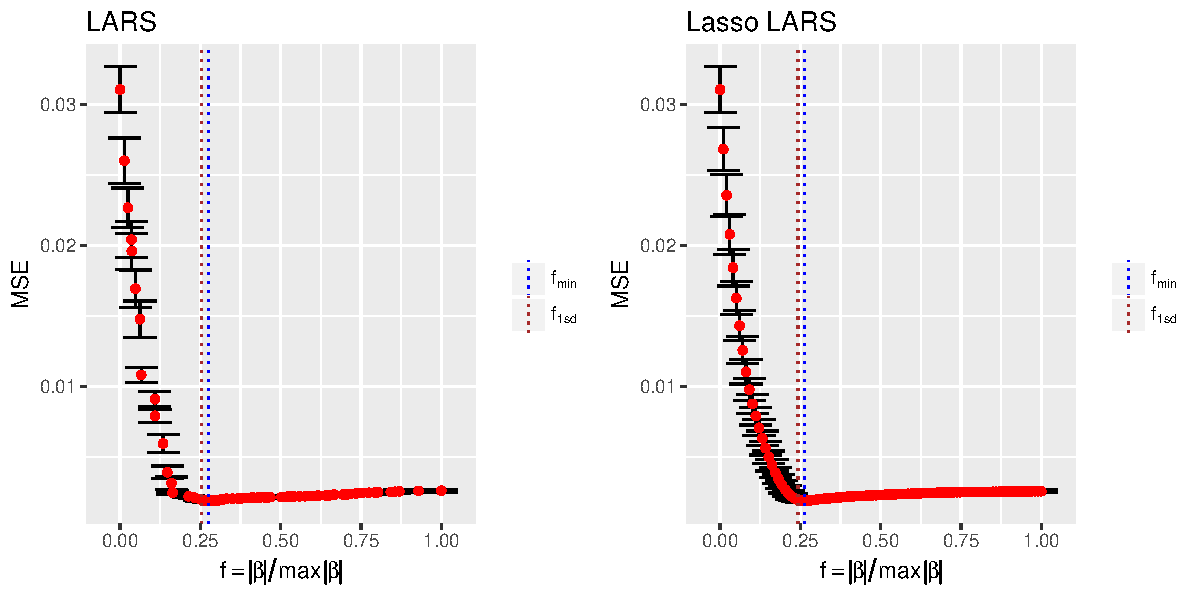
\includegraphics[width=1\linewidth, height=0.7\textheight]{slides/lars_kryds.pdf}
 \caption{10-fold krydsvalideringsfejl som funktion af fraktionen af \(\ell_1\)-normen LARS og lasso LARS.}
 \end{figure}
 %De stiplede linjer indikerer \(f_\text{min}\) og \(f_\text{1sd}\).
\end{frame}


\begin{frame}{LARS}{Krydsvalidering}
\begin{table}
\center
\scalebox{0.8}{
\begin{tabular}{lccccc | lccccc}
\toprule
 \multicolumn{6}{c}{LARS (CV) } & \multicolumn{1}{c}{ }&   \multicolumn{5}{c}{Lasso LARS (CV)}  \\ \midrule
& Værdi & MSE & $p$ &R$^2_{\text{adj}}$ &LogLik & & Værdi & MSE & $p$ & R$^2_{\text{adj}}$ & Loglike\\
%lars
$f_{\text{min}}$ & $0.2753$ &  0.0019 & 27 & 94.43\% & 974.8317 & 
%lasso min
\(f_{\min}\) &  0.2626 & 0.0019 & 21  & 94.52\% & 980.0982 \\
%lars sd
$\boldsymbol{f}_{\textbf{1sd}}$ & $\textbf{0.2542} $ & \textbf{0.0019} & \textbf{19} & \textbf{94.19}\%& \textbf{967.2669}
%lasso sd
&$\boldsymbol{f}_{\textbf{1sd}}$ & \textbf{0.2424} & \textbf{0.0019} & \textbf{13 } & \textbf{94.43}\% &  \textbf{971.6687} \\ \bottomrule
 \end{tabular}}
\caption{Værdien af $f_{\min}$ og $f_{1\text{sd}}$, gennemsnitlig krydsvalideringsfejl, som er målt i MSE, antallet af parametre, justeret R$^2$ og log-likelihood for LARS og lasso LARS. De valgte tuning parametre er markeret med tykt.} \label{tab:lars_lasso_tab}
\end{table}
\begin{itemize}
\item 22 trin udføres for lasso LARS (CV), hvor variablerne \textcolor{chartreuse4}{CUMFNS}, \textcolor{blue3}{MANEMP} og \textcolor{orange}{GS1} tilføjes og fjernes igen og 
variablen \textcolor{orange}{TB6MS} bliver tilføjet, fjernet og så tilføjet igen.  
\end{itemize}
\end{frame}

%\begin{frame}{LARS}{Krydsvalidering}
%\begin{figure}
%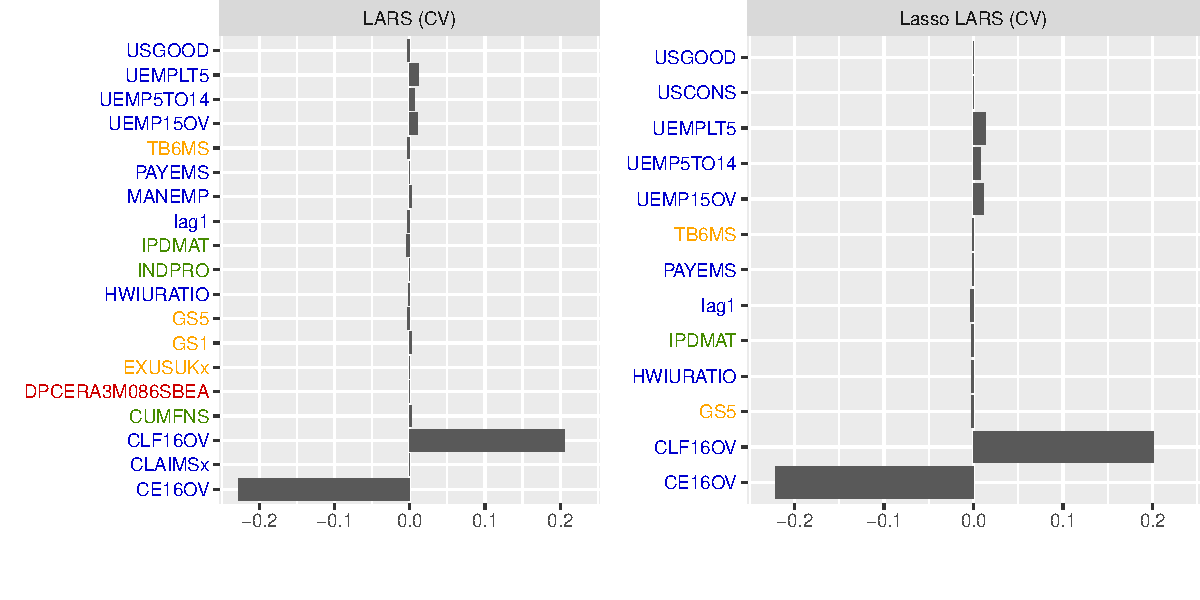
\includegraphics[width=1\linewidth, height=0.7\textheight]{slides/coef_lars_kryds.pdf}
%\caption{Estimerede koefficienter for LARS (CV) og lasso LARS (CV).}
%\end{figure}
%\begin{itemize}
%\item afviser normalitet samt at de første 10 autokorrelationer er nul
%\end{itemize}
%\end{frame}

\begin{frame}{LARS}{Krydsvalidering}
Bootstrap resultater af LARS (CV)
\begin{figure}
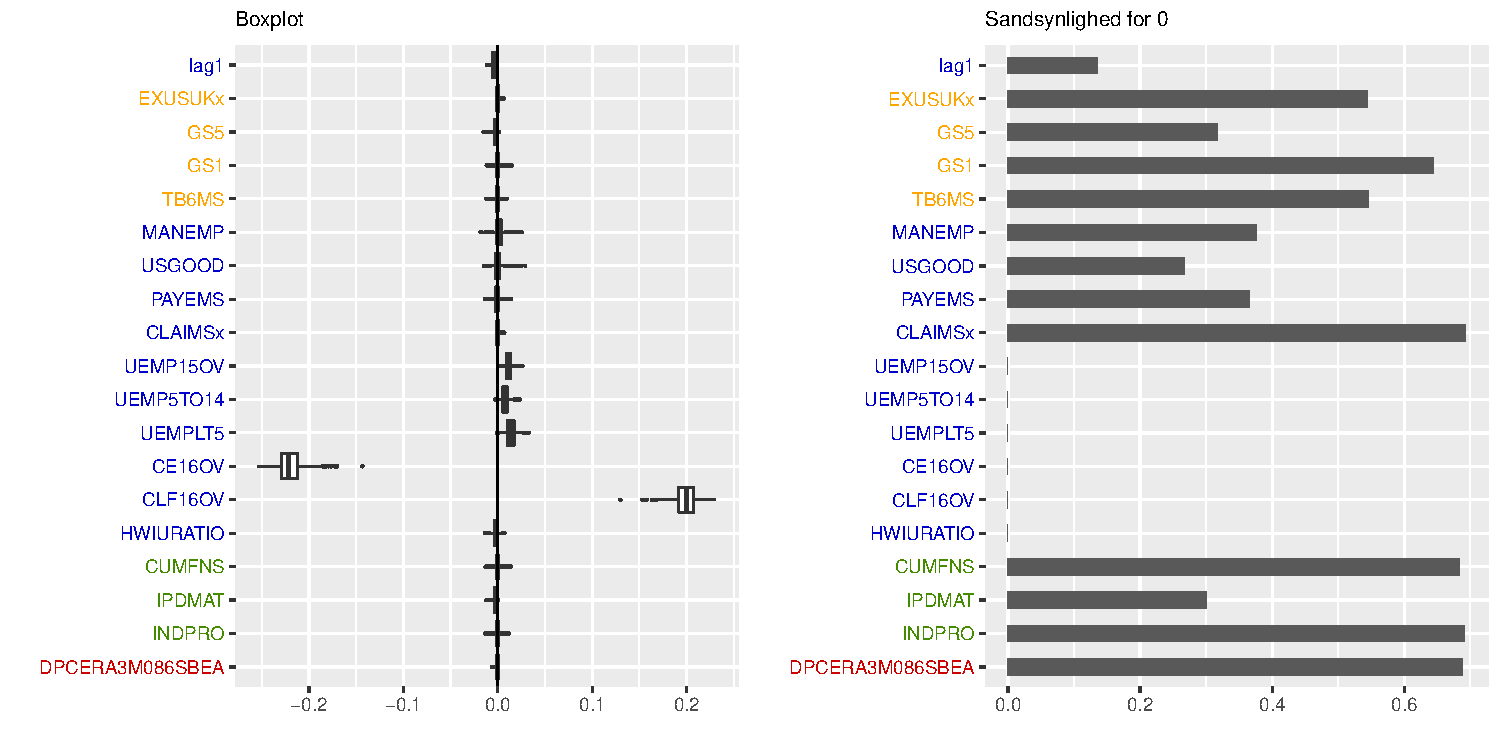
\includegraphics[width=1\linewidth, height=0.7\textheight]{slides/boxplot_lars_kryds.pdf}
%\caption{Til venstre vises et boxplot af 1000 bootstrap realisationer af $\widehat{\boldsymbol{\beta}}^{\text{LARS}} \del{f_\text{1sd}} $.
%Plottet til højre illustrerer andelen af bootstrap realisationer, hvor parameter estimaterne er præcis nul.}
\end{figure}
%\begin{itemize}
%\item afviser normalitet samt at de første 10 autokorrelationer er nul
%\end{itemize}
\end{frame}

\begin{frame}{LARS}{Krydsvalidering}
Bootstrap resultater af lasso LARS (CV)
\begin{figure}
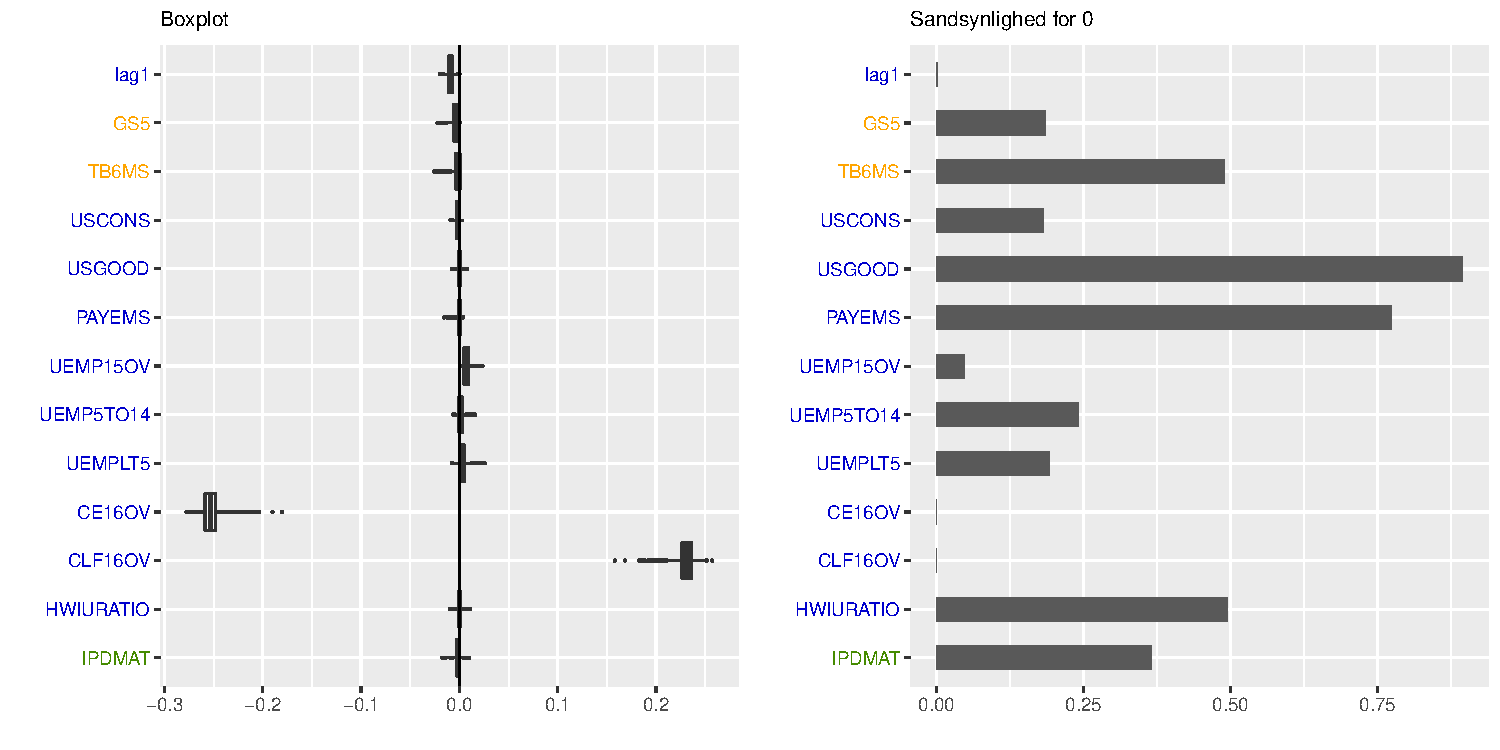
\includegraphics[width=1\linewidth, height=0.7\textheight]{slides/boxplot_lasso_kryds.pdf}
%\caption{Til venstre vises et boxplot af 1000 bootstrap realisationer af $\widehat{\boldsymbol{\beta}}^{\text{lasso}} \del{f_\text{1sd}} $.
%Plottet til højre illustrerer andelen af bootstrap realisationer, hvor parameter estimaterne er præcis nul.}
\end{figure}
%\begin{itemize}
%\item afviser normalitet samt at de første 10 autokorrelationer er nul
%\end{itemize}
\end{frame}

\begin{frame}{LARS}{Krydsvalidering}
\begin{table}[ht] 
\centering 
\scalebox{0.8}{
\begin{tabular}{lccc}
%\multicolumn{3}{l}{LARS algoritmen med lasso modifikation} \\
\toprule
Prædiktor & Cov test & \(p\)-værdi \\
\midrule
 \textcolor{blue3}{HWIURATIO}  &   864.6317 & 0 \\
 \textcolor{blue3}{UEMP15OV}  &   161.3770&  0 \\
 \textcolor{blue3}{UEMPLT5} &  163.0670 & 0 \\
 \textcolor{blue3}{UEMP5TO14}  &   122.3840  &0 \\
 \textcolor{blue3}{CE16OV} & 14.7416  &0 \\
 \textcolor{blue3}{PAYEMS} &  0.3356  &0.7151 \\
  \textcolor{blue3}{USGOOD}  &   5.0872 & 0.0066 \\
 \textcolor{blue3}{CLF16OV}    &   221.9181 & 0 \\
\textcolor{chartreuse4}{IPDMAT}       &    0.0668&  0.9354 \\
\textcolor{orange}{GS5}   &       0.3856 &    0.6803 \\
 \textcolor{blue3}{ lag1 }  &      0.8897 &    0.4115 \\
\textcolor{orange}{ TB6MS }&       0.0419   &  0.9590 \\
 \textcolor{blue3}{USCONS }&   0.0132   &  0.9869 \\ 
\bottomrule
\end{tabular}}
\caption{Kovarians testen for lasso LARS (CV).
Vi viser kun \(p\)-værdier for prædiktorer som medtages og bliver i modellen, dvs hvis en prædiktor medtages i et trin og senere forlader modellen, vises denne prædiktor ikke.
\(p\)-værdier \(< 2.2 \cdot 10^{-16}\) sættes lig 0.} \label{tab:covTest}
\end{table} 
\end{frame}

\begin{frame}{LARS}{Krydsvalidering}
\begin{table}[ht] 
\centering 
\scalebox{0.6}{
\begin{tabular}{lccccccc}
%\multicolumn{9}{l}{LARS algoritmen} \\
\toprule
Prædiktor& Koefficient & Z-score &\(p\)-værdi & Konfidensinterval &   $\sbr{\pazocal{V}^-,\pazocal{V}^+}$   \\
\midrule
\textcolor{blue3}{HWIURATIO}& 0.002  & 0.694   & 0.160    &  $\del{-\infty   ,  \infty}$   &$\sbr{0.002,0.002} $    \\
 \textcolor{blue3}{UEMP15OV} &    0.004&   1.606 & 0.923 &     $ \left( -\infty  ,  0.032\right] $     &$\sbr{0.004, 0.005}$   \\
 \textcolor{blue3}{UEMPLT5} & 0.001   &0.149   & 0.064  & $ \left[-0.018  ,     \infty\right) $  & $\sbr{0.000 ,0.001}$   \\
\textcolor{blue3}{MANEMP}   &   0.002 &  0.486   &0.273 &   $\left[-0.171 ,      \infty\right)$  & $\sbr{0.002,0.003}$\\
 \textcolor{blue3}{UEMP5TO14}  &$-  0.001$ & $-0.242 $ &0.077  &   $ \left( -\infty    ,  0.016\right] $&      $\sbr{0.000 ,0.001}$ \\
\textcolor{blue3}{CE16OV} &$- 0.267$ &$-37.446$ & 0.130   &   $\left( -\infty   ,  0.532\right]  $&    $\sbr{0.267, 0.267}$     \\ 
\textcolor{blue3}{ PAYEMS } &   0.000 &  0.006  & 0.563   &  $\del{-\infty ,  \infty}$   & $\sbr{0.000 ,0.000}$  \\
 \textcolor{blue3}{USGOOD} &$- 0.003$  &$-0.498$ &0.638   &   $\del{-\infty ,  \infty}$ &    $\sbr{0.003 ,0.003}$\\
\textcolor{chartreuse4}{CUMFNS} &  0.002  & 0.404 & 0.478    & $\del{-\infty   ,  \infty}$  &  $\sbr{0.002 ,0.002 }$  \\
 \textcolor{blue3}{CLF16OV} &  0.243  &36.643   & 0.179   &  $\del{-\infty  ,  \infty}$ &  $\sbr{0.243 ,0.243}$ \\  
\textcolor{chartreuse4}{ IPDMAT}& $-0.006$ &$ -1.626 $  &0.874   & $\left[-0.125  ,    \infty\right) $& $\sbr{0.006, 0.006}$ \\   
\textcolor{orange}{ TB6MS} & $-0.005$  &$-0.715$  & 0.569 &     $\del{-\infty  ,  \infty}$&   $\sbr{0.005, 0.006}$   \\ 
\textcolor{chartreuse4}{INDPRO} &  0.003 &  0.513  &0.328   &  $\del{-\infty   ,  \infty }$    & $\sbr{0.003 ,0.003}$  \\
\textcolor{orange}{GS1} &   0.006&   0.577    &0.473  &    $\del{-\infty  ,  \infty}$  &$\sbr{0.006 ,0.006}$ \\  
\textcolor{orange}{GS5} & $-0.005$ & $-1.146 $ &0.037 &     $\left( -\infty ,  -0.025\right]   $ & $\sbr{0.005 ,0.005 }$\\  
 \textcolor{blue3}{lag1}  & $-0.009$  &$-3.949$   & 0.910   & $\del{-\infty  ,  \infty }$  &$\sbr{0.009, 0.009 }$ \\ 
 \textcolor{red3}{DPCERA3M086SBEA} & $- 0.003$ & $-1.436$ & 0.233  &   $\del{-\infty   ,  \infty }$ &  $\sbr{0.003, 0.003}$ \\ 
\textcolor{orange}{ EXUSUKx}  &  0.003   &1.383 & 0.964   &   $\left( -\infty     ,-0.053 \right] $&  $\sbr{0.003, 0.003 }$   \\   
 \textcolor{blue3}{CLAIMSx} &0.002 &  0.813   & 0.226 &    $\del{-\infty  ,  \infty}$& $\sbr{0.002 ,0.002 }$   \\ 
\bottomrule
\end{tabular}  
}
\caption{Koefficienter, \(Z\)-scores, \(p\)-værdier, konfidensintervaller og trunkeret intervaller for LARS$_{TG}$ (CV). Den estimeres standard afvigelse er \(0.043\), og resultaterne er for \(f_{1 \text{sd}} = 0.2542\) med \(\alpha = 0.1\).} \label{tab:larInf_kryds}
\end{table} 
%\begin{itemize}
%\item afviser normalitet samt at de første 10 autokorrelationer er nul
%\end{itemize}
\end{frame}

%%%%%%%% BIC %%%%%%%%%
%\subsection{BIC}
%\begin{frame}{LARS}{BIC}
%\begin{table}
%\center
%\scalebox{0.8}{
%\begin{tabular}{lccccc| lccccc} 
%\toprule
%\multicolumn{6}{c}{LARS (BIC)}  & \multicolumn{6}{c}{Lasso LARS (BIC)} \\ \midrule
%& Værdi & BIC & $p$ & R$^2_{\text{adj}}$ & LogLik& & Værdi & BIC & $p$ & R$^2_{\text{adj}}$ & LogLik \\
%$f_\text{BIC}$ & 0.2623 & $-6.0925$ & 20 &94.43\% & 975.2909  &$f_\text{BIC}$ &  0.2604 &$-6.1627$& 17 &  94.46\% & 974.9938 \\ \bottomrule
% \end{tabular}}
%\caption{Værdien af $f_\text{BIC}$, antallet af parametre, BIC, justeret R$^2$  og log-likelihood for LARS og lasso LARS.} \label{tab:bic_lars}
%\end{table}
%\begin{itemize}
%\item 32 trin udføres for lasso LARS (BIC), hvor variablerne \textcolor{chartreuse4}{CUMFNS}, \textcolor{blue3}{MANEMP}, \textcolor{orange}{GS1}, \textcolor{blue3}{HWIURATIO}, \textcolor{blue3}{PAYMENS} og \textcolor{blue3}{USGOOD} tilføjes og fjernes igen og variablen \textcolor{orange}{TB6MS} bliver tilføjet, fjernet og så tilføjet igen. 
%\end{itemize}
%\end{frame}
%
%%\begin{frame}{LARS}{BIC}
%\begin{figure}
% 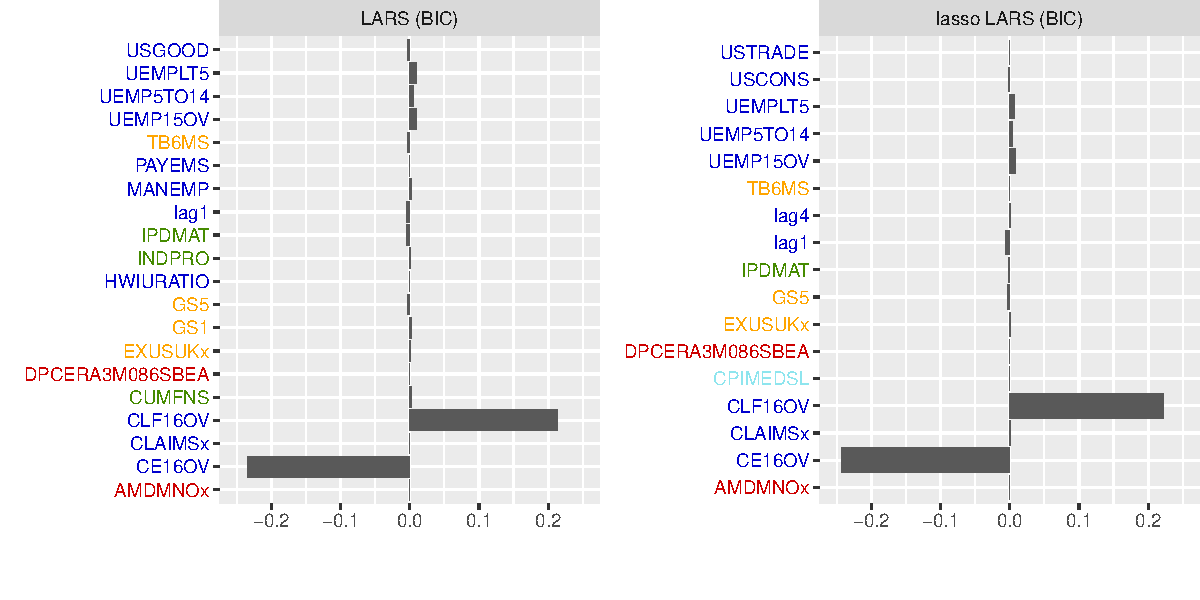
\includegraphics[width=1\linewidth, height=0.7\textheight]{slides/coef_plot_lars_bic.pdf}
% \caption{Estimerede koefficienter for LARS (BIC) og lasso LARS (BIC).}
% \end{figure}
% \begin{itemize}
%\item afviser normalitet samt at de første 10 autokorrelationer er nul
%\end{itemize}
%\end{frame}
%
%\begin{frame}{LARS}{BIC}
%\begin{figure}
% 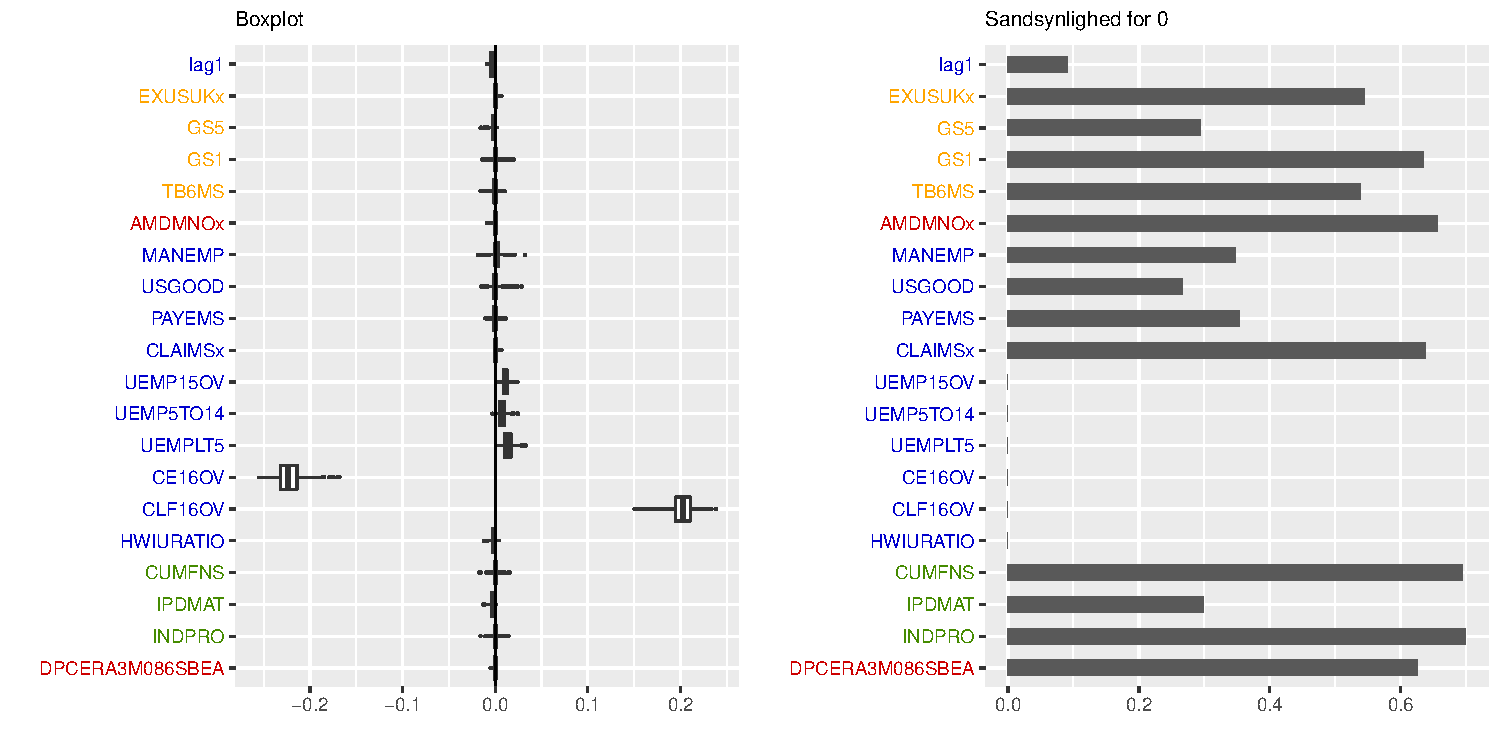
\includegraphics[width=1\linewidth, height=0.7\textheight]{slides/boxplot_lars_bic.pdf}
% \caption{Til venstre vises et boxplot af 1000 bootstrap realisationer af $\widehat{\boldsymbol{\beta}}^{\text{LARS}} \del{f_\text{BIC}} $.
%Plottet til højre illustrerer andelen af bootstrap realisationer, hvor parameter estimaterne er præcis nul.}
% \end{figure}
% \begin{itemize}
%\item afviser normalitet samt at de første 10 autokorrelationer er nul
%\end{itemize}
%\end{frame}
%
%
%\begin{frame}{LARS}{BIC}
%\begin{figure}
% 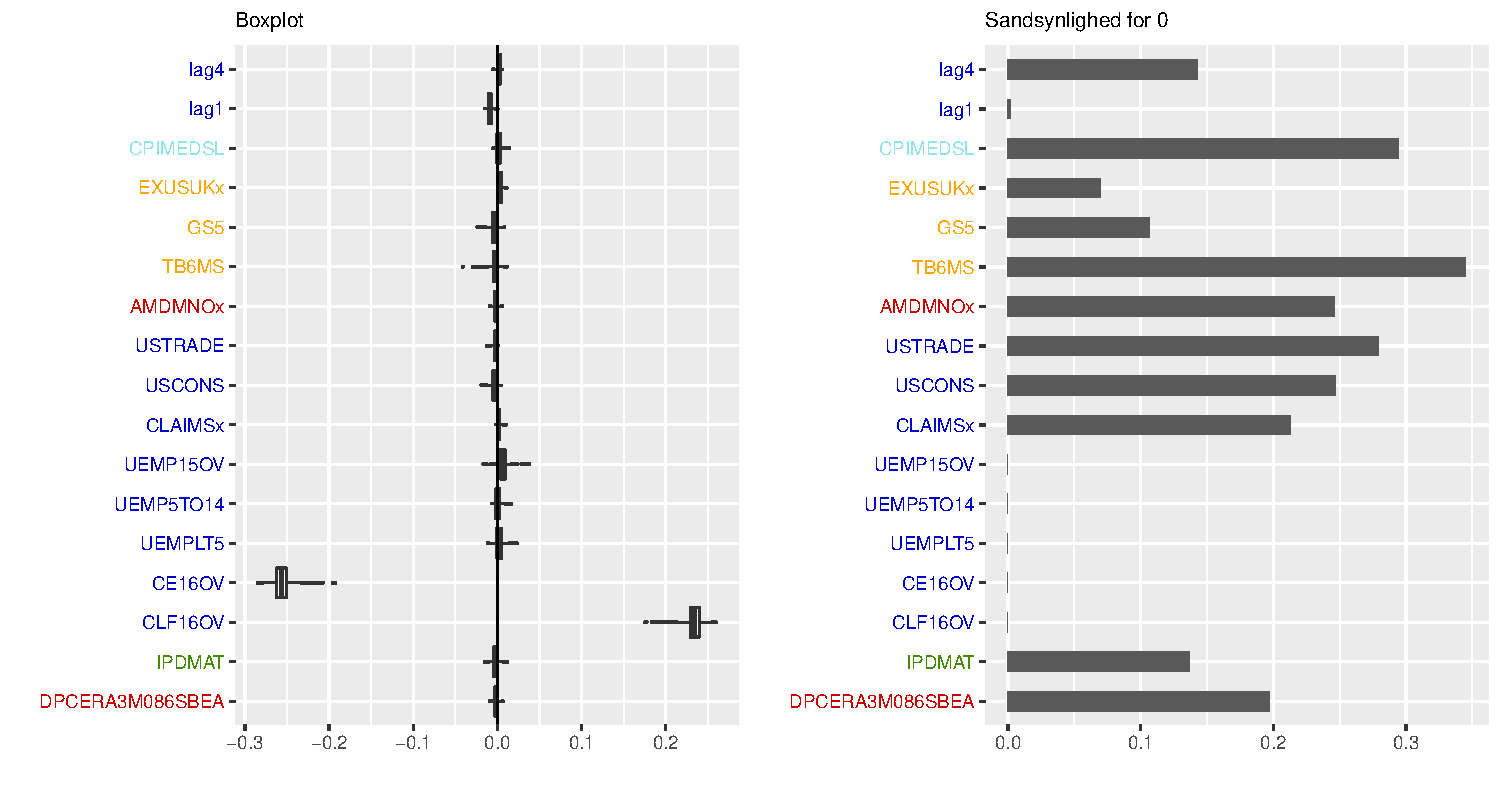
\includegraphics[width=1\linewidth, height=0.7\textheight]{slides/boxplot_lars_lasso_bic.pdf}
% \caption{Til venstre vises et boxplot af 1000 bootstrap realisationer af $\widehat{\boldsymbol{\beta}}^{\text{lasso}} \del{f_\text{BIC}} $.
%Plottet til højre illustrerer andelen af bootstrap realisationer, hvor parameter estimaterne er præcis nul. }
% \end{figure}
% \begin{itemize}
%\item afviser normalitet samt at de første 10 autokorrelationer er nul
%\end{itemize}
%\end{frame}
%
%\begin{frame}{LARS}{BIC}
%\begin{table}[ht] 
%\centering 
%\scalebox{0.6}{
%\begin{tabular}{lccc}
%\multicolumn{3}{l}{LARS algoritmen med lasso modifikation} \\
%\toprule
%Prædiktor & Cov test & \(p\)-værdi \\
%\midrule
%\textcolor{blue3}{UEMP15OV}    &       161.3770  &0\\
%\textcolor{blue3}{UEMPLT5}   &      163.0670 & 0\\
%\textcolor{blue3}{UEMP5TO14}    &    122.3840&  0\\
%\textcolor{blue3}{CE16OV}         &   14.7416 & 0\\
%\textcolor{blue3}{CLF16OV}        &   221.9181 & 0\\
%\textcolor{chartreuse4}{IPDMAT}         &    0.0668&  0.9354\\
%\textcolor{orange}{GS5}&   0.3856 & 0.6803\\
%\textcolor{blue3}{lag1}       &      0.8897 & 0.4115\\
%\textcolor{orange}{TB6MS}  &    0.0419 & 0.9590\\
%\textcolor{blue3}{USCONS} &    0.0132&  0.9869\\
%\textcolor{red3}{ DPCERA3M086SBEA}          &  0.0254 & 0.9750\\
%\textcolor{orange}{ EXUSUKx} &     0.2309 & 0.7939\\
%\textcolor{blue3}{CLAIMSx} &      0.0082 &  0.9919\\
%\textcolor{red3}{ AMDMNOx}  &     0.0464 & 0.9546\\
%\textcolor{blue3}{lag4 }     &    0.2281&  0.7962\\
%\textcolor{cadetblue2}{CPIMEDSL}  &   0.0719&  0.9307\\
%\textcolor{blue3}{USTRADE}   &     0.0029 &  0.9971\\ \bottomrule
%\end{tabular}}
%\caption{Kovarians testen for lasso LARS (BIC).
%Vi viser kun \(p\)-værdier for prædiktorer som medtages og bliver i modellen, dvs hvis en prædiktor medtages i et trin og senere forlader modellen, vises denne prædiktor ikke.
%\(p\)-værdier \(< 2.2 \cdot 10^{-16}\) sættes lig 0.} \label{tab:covTest_bic}
%\end{table} 
%\end{frame}
%
%\begin{frame}{LARS}{BIC}
%\begin{table}[ht] 
%\centering 
%\scalebox{0.6}{
%\begin{tabular}{lcccccc}
%\multicolumn{9}{l}{LARS algoritmen} \\ 
%\toprule
%Prædiktor&  Koefficient & Z-score  & \(p\)-værdi & Konfidensinterval& $\sbr{\pazocal{V}^-,\pazocal{V}^+}$   \\ \midrule
%\textcolor{blue3}{HWIURATIO} &0.002  & 0.720   &0.161    &   $\del{-\infty   ,  \infty }$ &  $\sbr{0.002,0.002}$    \\
% \textcolor{blue3}{UEMP15OV} & 0.004  & 1.596  4 &  0.920 &     $\left( -\infty  ,      0.034 \right] $& $\sbr{0.004 ,0.005}$  \\
%\textcolor{blue3}{UEMPLT5}  & 0.001 &  0.148   & 0.065  & $\left[-0.018    ,    \infty  \right)$   &$\sbr{0.000,0.001}$    \\
%\textcolor{blue3}{MANEMP} &0.003 &  0.561    & 0.766 &       $\left(  -\infty     ,  0.120\right] $ &$\sbr{0.003, 0.003}$  \\
% \textcolor{blue3}{ UEMP5TO14} & 0.001 & $-0.261$ &  0.093   &  $\left( - \infty    ,  0.023\right] $&   $\sbr{0.000, 0.001}$ \\
%\textcolor{blue3}{ CE16OV}   & $-0.267 $& $-37.412$  & 0.130  &    $\left( -\infty     ,   0.574\right] $  &$\sbr{0.266, 0.267}$ \\
% \textcolor{blue3}{PAYEMS} &  0.000  & 0.012  & 0.428  &    $\del{-\infty   ,  \infty }$ &  $\sbr{0.000 ,  0.000}$   \\
% \textcolor{blue3}{USGOOD} & $-0.004$ & $-0.584$ & 0.721   &   $\del{-\infty   ,  \infty } $&    $\sbr{0.004 ,  0.004   }$   \\
%\textcolor{chartreuse4}{CUMFNS} &  0.002   &0.390  & 0.455     &  $\del{-\infty   ,  \infty }$& $\sbr{0.002 ,  0.002 }$   \\
% \textcolor{blue3}{ CLF16OV}  &   0.243 & 36.646   &  0.179    &  $\del{-\infty   ,  \infty }$&$\sbr{0.243 ,  0.243}$    \\
%\textcolor{chartreuse4}{ IPDMAT}& $-0.006$ & $ -1.618$   & 0.869  & $\left[ -0.130  ,      \infty  \right)$&   $\sbr{0.006,   0.006}$     \\
% \textcolor{orange}{TB6MS}& $-0.006$ & $-0.790 $  & 0.615     &  $\del{-\infty   ,  \infty } $  & $\sbr{0.006 ,  0.006}$   \\
% \textcolor{chartreuse4}{INDPRO}&   0.003   &0.591   & 0.494  &    $\del{-\infty   ,  \infty }$ &  $\sbr{0.003,   0.003}$    \\
% \textcolor{orange}{GS1} &  0.007&   0.675  & 0.571 &      $\del{-\infty   ,  \infty }$ &   $\sbr{0.007 ,  0.007}$     \\
% \textcolor{orange}{GS5} &   $-0.006$ &$ -1.240$  & 0.302&      $\del{-\infty   ,  \infty }$&   $\sbr{0.006,  0.006}$   \\
% \textcolor{blue3}{lag1} & $-0.009$ & $ -3.914  $  &  0.912   &  $\del{-\infty   ,  \infty }$& $\sbr{0.009,   0.009 }$   \\
%  \textcolor{red3}{DPCERA3M086SBEA}   & $-0.002$ &  $-1.331  $ & 0.225 &      $\del{-\infty   ,  \infty }$& $\sbr{0.002,   0.002 }$   \\
% \textcolor{orange}{EXUSUKx} & 0.003 &  1.357   & 0.964  &    $\left( -\infty   ,  -0.051\right] $&  $\sbr{0.003 ,  0.003}$   \\
% \textcolor{blue3}{CLAIMSx} &  0.001  & 0.629  & 0.208   &   $\del{-\infty   ,  \infty }$ & $\sbr{ 0.001 ,  0.001 }$  \\
% \textcolor{red3}{AMDMNOx} &  $-0.002$ &  $-0.904 $   & 0.855     &  $\del{-\infty   ,  \infty }$&$\sbr{0.002 ,  0.002}$  \\ \bottomrule
%\end{tabular}  
%}
%\caption{Koefficienter, \(Z\)-scores, \(p\)-værdier, konfidensintervaller og trunkeret intervaller for LARS$_{TG}$ (BIC). Den estimeres standard afvigelse er \(0.043\), og resultaterne er for \(\widehat{f}_{\text{BIC}} = 0.2623 \) med \(\alpha = 0.1\).} \label{tab:larInf_bic}
%\end{table} 
% \begin{itemize}
%\item afviser normalitet samt at de første 10 autokorrelationer er nul
%\end{itemize}
%\end{frame}


%%% Local Variables:
%%% mode: latex
%%% TeX-master: "../beamer"
%%% End:
